
\part{Guarantee AI : Composition of Strategies}

    \section{Description}
    
    For the guaranteed AI we decided to extend what we had already begun to implement during the PD/GL course, which is the Strategy pattern.
    We created different types of strategy for every action (or category), each one being specialized in one type of decision. For each type we can create a player that focuses on one thing. For example crystallizing as much as possible, trying to summon as many cards as possible, or more complex choices like focusing on using combos.
    With that in place, we could create a way to compose a player's strategy, so it could adapt its way of "thinking" depending on the context by switching from a strategy to another.
    The context under which a player must use a strategy or not is defined when we create the player and add the strategy. If the context associated with the strategy is respected, then the said strategy is applied. Else it switches to the next strategy we gave him.
    
    \section{Strategies}
    
    During a game of Seasons, the player has a lot of choices to make and they are very different, he may choose a dice, a card or decide what to do during his turn.
    With that in mind, we decided to implement different types of choice, in order to make good strategies for each type of choice.
    
    
    \subsection{Shape of a strategy}
    
        An abstract strategy contains two fields: a \textbf{nextStrategy} of the same type and a Context \textbf{context}.
        It contains a method \textbf{doChoose}, which is the one that is called in order to use the strategy. It checks if the context is corresponding, and if it does it calls the method \textbf{choose} which actually makes the choice. This method can either return the choice of the player or a \textit{null}.
        If the context does not correspond or if the method \textbf{choose} returns \textit{null}, the method \textbf{doChoose} of \textbf{nextStrategy} is called.
        
        The strategies of a same category extend the corresponding abstract strategy and override the method choose which allows us to define different kinds of choice.
    
    \newpage
    \subsection{Categories of strategy}
    
        \paragraph{ChooseBonus}
        This category contains the strategies defining how a player will decide which bonus to choose from those available.
        
        \paragraph{ChooseCardBetweenMultipleToGet}
        This category contains the strategies defining which card a player will keep when choosing between several different cards. It is used with the bonus allowing to draw two cards, the cards \textit{Divine Chalice} and \textit{Amulet of Fire}.
        
        \paragraph{ChooseCardComeBackInHand}
        This category contains the strategies defining which card to choose from the player's board which is going to come back in his hand. It is used with the effect of the card \textit{Amsug Longneck}.
        
        \paragraph{ChooseCardForInitHand}
        This category of strategies contains every way of choosing how the player wants to organize his cards for the different years at the beginning of the game.
        
        \paragraph{ChooseCardNariaLaProphetesse}
        This category of strategies contains every way of choosing which card to keep and which card to give to the other players when using the card \textit{Naria The Prophetess}.
        
        \paragraph{ChooseCardToDelete}
        This category contains the strategies defining how the player will choose the card to sacrifice when a player uses the card \textit{Syllas The Faithfull}.
        
        \paragraph{ChooseCardToSummon}
        This category contains the strategies defining how a player will choose which card he will summon from his hand.
        
        \paragraph{ChooseCardToSummonForFree}
        This category contains the strategies defining how a player will choose which card he will summon from his hand for free. It is used when the player sacrifices the card \textit{Potion Of Dream}.
        
        \paragraph{ChooseCardToActivate}
        This category contains the strategies defining how a player will choose which card he will activate from his board.
        
        \paragraph{ChoosePlayerEnergyToCopy}
        This category contains the strategies defining how a player will choose another player in order to copy his stock of energies when using the card \textit{Lewis Greyface}. 
        
        \paragraph{ChooseDice}
        This category contains the strategies defining how a player will choose a die between the dice proposed in the game on every turn. 
        
        \paragraph{ChooseEnergyToCrystallize}
        This category contains the strategies defining how a player will choose the energy from his stock he will crystallize.
        
        \paragraph{ChooseEnergyToGet}
        This category contains the strategies defining how a player will choose which energy to get. It is used with the cards \textit{Beggar's Hom}, \textit{Bespelled Grimoire}, \textit{Potion Of Knowledge}, \textit{Hourglass Of Time}, \textit{Yjang's Forgotten Vase}, \textit{Amulet Of Water} and the bonus which allows to exchange an energy for another.
        
        \paragraph{ChooseEnergyToReduce}
        This category contains the strategies defining how a player will choose which energy to remove from the cost of a card, which is the effect of the card \textit{Hand Of Fortune}.
        
        \paragraph{ChooseEnergyToThrow}
        This category contains the strategies defining how a player will choose which energy to throw out of his energy stock. It is used when a player earns an energy but has a full energy stock, with the card \textit{Kairn The Destroyer} when he has to spend an energy, and with the bonus which permits to exchange an energy for another.
        
        \paragraph{ChooseNbDeplacementSeason}
        This category contains the strategies defining how a player will decide where he wants to move when he uses the card \textit{Temporal Boots}. This strategy uses strategy ChooseGoToTheNextSeason, ChooseGoToThePreviousSeason and ChooseStayInTheSeason.
        
        \paragraph{ChooseStayInTheSeason}
        This category contains the strategies defining how a player will decide if he want to stay in the actual season.
        
        \paragraph{ChooseGoToTheNextSeason}
        This category contains the strategies defining how a player will decide if he want to go in the next season.     
        
        \paragraph{ChooseGoToThePreviousSeason}
        This category contains the strategies defining how a player will decide if he want to go in the previous season.  
        
        \paragraph{ChoosePlayerAction}
        This category contains the strategies defining how a player will choose which action he should do during his turn.
        
        \paragraph{ChooseSimilarEnergyToDelete}
        This category contains the strategies defining how a player will choose which type of energy to delete when the player has to delete several energies of a same type. It is used when the player uses the card \textit{Balance Of Ishtar}.
        
        \paragraph{ChooseToKeepDrawnCard}
        This category contains the strategies defining how a player will choose whether he keeps the card he has drawn or not. It is used a the begin of the turn of the player if he has the option to draw a card on his die.
        
        \paragraph{ChooseToUseBonusCard}
        This category contains the strategies defining how a player will decide if he chooses to use the bonus "draw two cards instead of one" when he gets the card from the die at the beginning of his turn. 
        
        \paragraph{ChooseUseDeDeLaMalice}
        This category contains the strategies defining how a player will decide if he uses the card "Die of Malice" when he has it on his board, at the beginning of his turn.
        
    \newpage
    \section{Comparator}
        Most of the time, when we implements strategies we need to compare different objects in order to determine which is the better. So to facilitate this comparison we creates multiples classes implementing Comparator.
        We have multiple type of comparator such as one which compare how much prestige point a card can give, which card is the best given by a list of the best card, etc...
        
        Alongside we also make some classes (singleton) which contains methods to compare more precisely. This classes are mostly used to compare card or energies with predefined list, like a list of energies sort by the most expensive in the actual season.
        
    
    
    \section{Player Factory}
        We created a Factory in order to create different types of AI easily. When we call the method \textbf{getPlayer(playerType, name)} of an object \textit{PlayerFactory}, the method creates a player with a strategy making random choices for each category. Then we enter a switch case which will set some (if not every) strategies to a different one according to the \textit{TypeAIPlayer} given in parameters.
        For example : \textbf{player.setChooseDice(new ChooseDicePrefCristallize())}
    
    
    \section{Context}

        \textit{IContext} is a class which represents an object containing a lambda expression. It contains a function \textbf{isVerified()} which triggers the contained lambda expression.
        Context is a container class, it stores static variables of type \textit{IContext} which contain a lambda expression with a Player as parameter.
        When we call the method \textbf{isVerified()} on a variable contained in the class Context, it gives us the result of the lambda expression.
        It allows us to get information about the game only by using this method.
        
        If we want to know if a player has more than 6 energies, we create the variable \textbf{static IContext moreThan6Energies = (player) -$>$ player.getFacadeIA().getEnergyStock().size() $>$= 6;} and then call \textbf{moreThan6Energies.isVerified()}.
        
        The contexts are used to know details about the advancement of the game and determine if a strategy should be used or not.
            
    \newpage
    \section{Implementation of players not composed}
    
        A player which is not composed always follows the same type of strategy.
        Every strategy implemented in the different categories aim to the same purpose.
        For example \textit{ChooseDicePrefCrystallize} will choose a die which gives the right to crystallize and \textit{ChoosePlayerActionPreCrystallize} will choose the action \textit{Crystallize} if it is available can.
        
            \paragraph{Choose First}
            This player only chooses the first choice from all those available. Mostly used during the development to test some methods.
            
            \paragraph{Random}
            This player makes every choice randomly no matter what.
            
            \paragraph{Pref Crystallize}
            This player chooses whatever can earn him crystals immediately.
            
            \paragraph{Pref Card Point}
            This player will always try to get as many points as possible at the end of the game, mainly by summoning cards with a high prestige point value.
            
            \paragraph{Pref Invocation}
            This player will always try to summon as many cards as possible.
            
            \paragraph{Combos}
            This player will attempt to form combos with his cards and his actions.
            
            \paragraph{Malus}
            This player chooses actions which can handicap other players, for example summon a card which will steal their energy. 
            
            \paragraph{Time Random}
            Time strategy will do everything to play with time, thanks to a die. Its choice between going forward or backward is random.
            
            \paragraph{Time First}
            Time First strategy will always try to stay in the current season.
            
            \paragraph{Time Crystallize}
            Time Crystallize will always try to be in the season in which its energies will be the most valuable.
            
            \paragraph{Time Invocation}
            Time Invocation will try to go forward if its hand is empty and backward otherwise.
            
            \paragraph{Activate}
            This player will try to activate his cards on his board every time he can.
            
            \paragraph{Pref Permanent}
            This player will use cards with a permanent effect as much as possible. A permanent effect can triggered during the whole game (for example each seasons, each end of turn).
        
        \section{Implementation of players composed}
        
        \subsection{Composition on the player factory}
                
            The goal of the composition is to use certain strategies in a certain context, and use some other in a different context, or if the first strategy doesn't give result, use the next one.
            
            In order to do this, when we create a player on the \textit{PlayerFactory} we can set a type of strategy with a composition of different types of strategies.
            A composed strategy look like:

            
            \paragraph{Strategy1()}
                When the strategy is created like this, the player will always use the strategy1.
                If this strategy doesn't return a result, the Random Strategy will be use.
            
            \paragraph{Strategy1( Context1, Strategy2())}
                When the strategy is created like this, the player will check if the context1 is verified, if it's the case the Strategy1 will be used, if not the Strategy2 will be applied.
                If the context1 is verified and the strategy1 doesn't give any result the strategy2 will be used.
            
            \paragraph{Strategy1(Strategy2())}
                Created that way, the player will always try to use the Strategy1. If it doesn't return any result, the Strategy2 will be applied.
            
            \paragraph{How does it work}
            The inheritance of a type of strategy is like this:
            
            \begin{figure}[H]
                \centering
                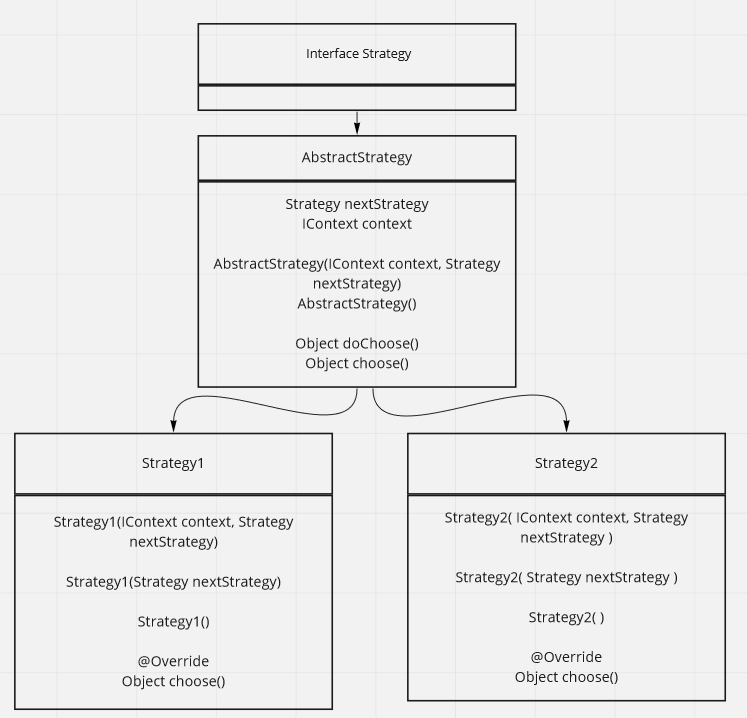
\includegraphics[scale=0.42]{rapport/images/graphics/graph_strategy.png}
                \caption{Schema of the inheritance of a strategy}
            \end{figure}
            
            
            When a choice is required from the player, he will call the method doChoose() in the first strategy in the corresponding composition.\\
            
            \underline{Strategy1()}: \textbf{doChoose()} will call the method \textbf{choose()}, which will return a result to \textbf{doChoose()} which will then return the result to the game. \\
            
            \underline{Strategy1(Strategy2())}: \textbf{doChoose()} of strategy1 will call the method choose() of strategy1.
            If this method return a result, \textbf{doChoose()} of strategy1 will return its result to the game, if not it will call the \textbf{doChoose()} of strategy2 which will then ask a result to the choose() method of strategy2.\\
            
            \underline{Strategy1 (context1, Strategy2())}: \textbf{doChoose()} of strategy1 will verify the context, if is is respected, \textbf{choose()} from strategy1 will be called. Else it will call \textbf{doChoose()} of strategy2.
            
        
            % faire une list ou alors mettre une petit explication sur ce que vous avez voulu faire comment vous avez fait
            \subsection{Compose Raph}
            The initial goal of this AI was to try to create a behavior as close as possible from that of a human. It is using a lot of contexts associated with strategies that would theoretically fit. This AI is detailed in the part \ref{compose_raph_appendix} of the appendix here
            
            
            \subsection{Compose Dyl}
            
            For this composition we try to humanized the AI to make specific choices at certain moment of the game for example we would like to choose a specific dice at the year 1 or 2 or activate the card \textit{Temporal boots} if we are at the last year.  \\
            We tried to adapt the AI behavior against others player but with static choice we could not get the better choice every time because this is a sequence of test that verified the context or not. 
            The AI make choice according to us human, what we would have done if we were playing, we saw by playing ourselves that some moves were better than other. For more details about each strategy and how is it composed see \ref{appendix:compose_dyl_appendix} 
            
            
            
            \subsection{Compose Marg}
            This composition try to reproduce the style of game of Margaux. This player is based on the strategies Pref Card Point and Pref Invocation because they limited the penalty cards at the end of the game. He try to played a little with the time only if he's in the last time to slow down or speed up in function of this hand and he don't crystallized except if is in the last year and last season. We try to arrange strategy to make the best possible player. The players strategies are detailed in the appendix \ref{appendix:compose_marg}.
            
    \newpage
    \section{Performance}
        
        \subsection{How to measure the performances}
            Most of the time when we test our AI we simply run a lot of games with two players and look at the percentage of victory of each player. Sometimes we also look at the number of prestige point gained during a game.
            At first, the games were played against the Random AI, then we eventually used more advanced AI like PrefCardPoint.
            After these tests, we run other games against 3 other AIs to see if the AI is also working and good on a game with 4 players and not only 2.

        \subsection{Not compose AI}
            Our goal with this kind of AI was to make strategies in order to create a great composed AI. We were quite surprised when we saw some of them have a good win rate against the Random AI. For example PrefCardPoint, PrefInvocation and Activate are quite good by themselves as we can see on the figure \ref{fight_images_not_compose_ia}. 
            
            Their efficiency can be explained by the fact that they're using cards more than the other AIs, which results in them having more cards on their boards and less in their hand. In the end they gain more points from their board and lose less from their hand.
            
            We tried different fights between all of our AIs but PrefCardPoint is undoubtedly the best one as shown on the figure \ref{fight_best_img}.

            \begin{figure}[H]
                \centering
                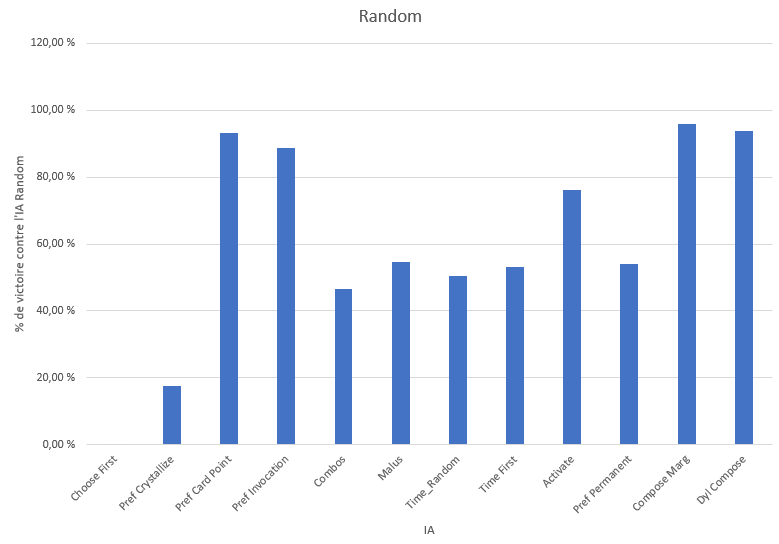
\includegraphics[scale=0.53]{rapport/images/graphics/Guaranteed_IA_against_random.png}
                \caption{Percentage of victory against the Random AI on 10000 games}
                \label{fight_images_not_compose_ia}
            \end{figure}
            
            \begin{figure}[H]
                \centering
                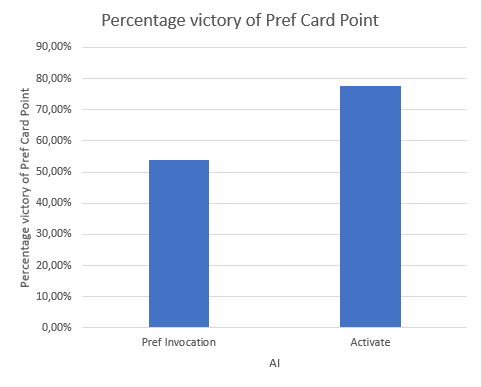
\includegraphics[scale=0.9]{rapport/images/graphics/fight_prefCard_Point.png}
                \caption{Percentage of victory against Pref Card Point}
                \label{fight_best_img}
            \end{figure}
            
        \subsection{AI composed}
            After seeing the performances of the AI which are not composed, it was a bit stressful to make a better AI than PrefCardPoint with a win-rate of 93\% against Random.
            
            
            But with a lot of tests, by composing and modifying each category of strategies, we successfully improved our AI as the figure \ref{fight_against_pref_card_point} highlights, representing the percentage of victory of the composed AI against the AI PrefCardPoint.
            With a win-rate already high for PrefCardPoint the gap is not very big but it is significant enough to see there is an upgrade.
            We tested this strategy against Random, PrefCardPoint and multiple different strategies.
            
            As we can see on the figure \ref{fight_composed_against_other} the composed AI are very efficient, 95\% of victory against random. But also our composed AI are slightly better than the best AI which are not composed, for example ComposeMarg has 57\% of victory against PrefCardPoint. It is not really high but quite good looking at our performance of PrefCardPoints in the figure \ref{fight_images_not_compose_ia}.  
            
            \begin{figure}[H]
                \centering
                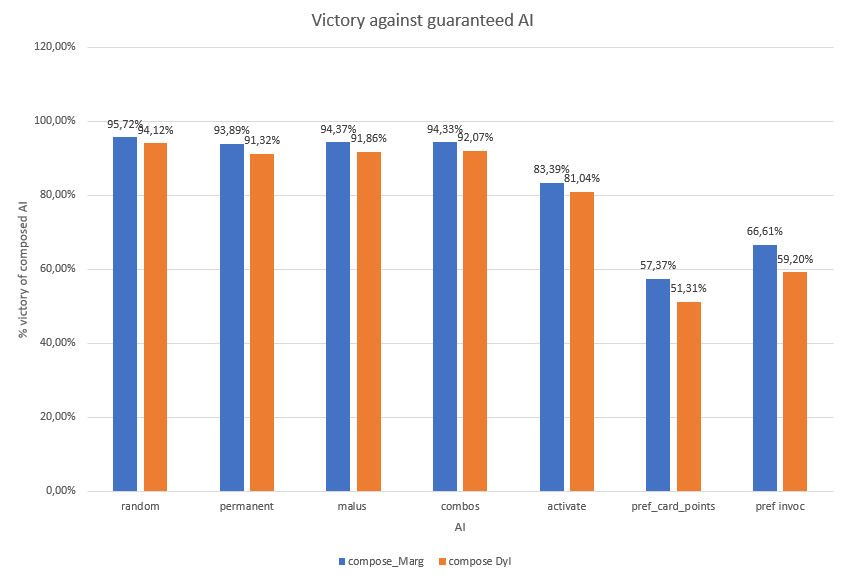
\includegraphics[scale=0.7]{rapport/images/graphics/fight_composed_guaranteed_ai.png}
                \caption{Percentage of victory of Compose Marg and Dyl Compose against other guaranteed AI}
                \label{fight_composed_against_other}
            \end{figure}
            
            \begin{figure}[H]
                \centering
                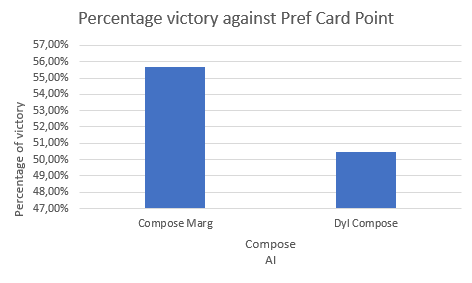
\includegraphics[scale=0.9]{rapport/images/graphics/fight_prefCardPoint_against_composed.png}
                \caption{Percentage of victory against Pref Card Point}
                \label{fight_against_pref_card_point}
            \end{figure}
            
             \begin{figure}[H]
                \centering
                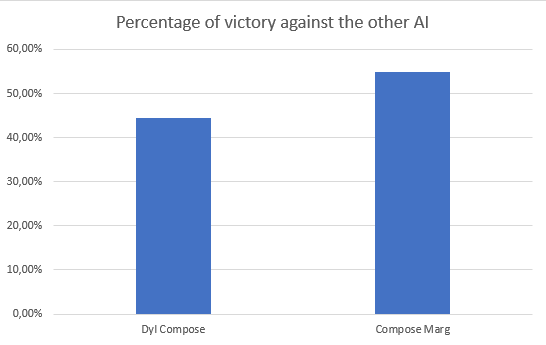
\includegraphics[scale=0.9]{rapport/images/graphics/fight_compose_marg_dyl.png}
                \caption{Percentage of victory against each other}
                \label{fight_compose}
            \end{figure}

    \section{Conclusion of Guarantee AI}
        We took a lot of time developing the guaranteed AI, it wasn't particularly difficult but rather long to implement. We made a lot of different strategies and tried to generalize it as much as we could, which was really time-consuming.
        But at the end the outcome was worth it. We have multiple guaranteed AI which are very good against the random one.
    